\chapter{The Development Environment}

In order to develop on a personal computer, must certain steps be performed in various systems, as well as various programs installed and configured. In this chapter these items will be discussed.

\section{Local Web Server Installation and Configuration}

In order for a locally developed project to be deployed, and to guarantee access to all required components a web server must be installed locally. 

\subsection{XAMPP}

In the iCampus web development group we use XAMPP from Apache Friends for our local web servers. Apache Friends describes XAMPP as follows:

\begin{quote}
	\textit{XAMPP is a completely free, easy to install Apache distribution containing MySQL, PHP, and Perl. The XAMPP open source package has been set up to be incredibly easy to install and to use.}\footnote{\url{https://www.apachefriends.org/index.html} September 19, 2014}
\end{quote}

\noindent
As per the description the distributions of XAMPP available from \href{https://www.apachefriends.org/index.html}{Apache Friends} come included with various useful tools which are also used within iCampus, such as PHP (server-side scripting language)abd MySQL (database management system), as well as many other tools which are optional for iCampus such as FileZilla (FTP Server) and Mercury (Mail Server).\\
\\
Download and install the latest XAMPP installation. Keeping in mind that at least MySQL and phpMyAdmin need to be installed to function in the iCampus environment.

\begin{figure}[h] 
	\centering
	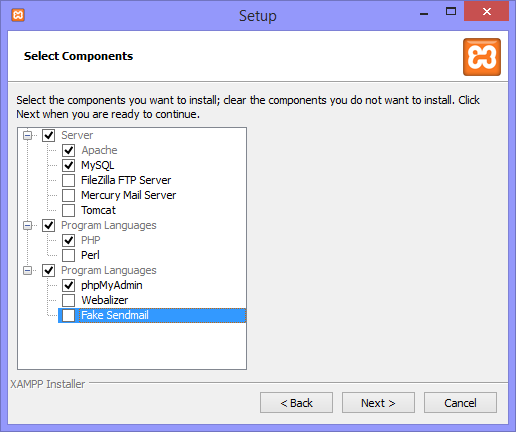
\includegraphics[width=6cm]{xampp.png}
	\caption{XAMPP Minimum Installation}
\end{figure}

\newpage
\subsection{PHP Configuration}
\label{subsec:phpconfig}

The next step is the configuration of PHP for error reporting using xdebug. To do this open your php.ini file using the XAMPP control panel or the file explorer. This file is typically located at \url{C:/xampp/php/php.ini}.\\

\begin{figure}[h] 
	\centering
	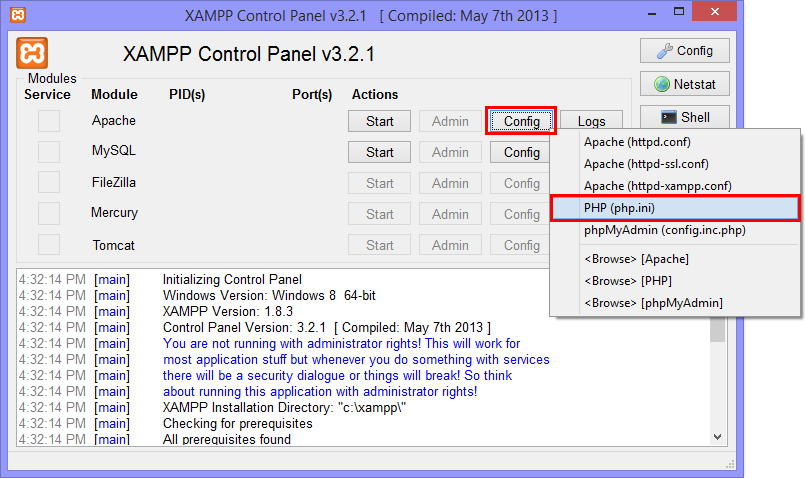
\includegraphics[width=6cm]{openphpini.png}
	\caption{XAMPP Control Panel}
	\label{fig:xamppcontrolpanel}
\end{figure}

The following modifications should then be made to the file:\\
\\

\begin{tabular}{l}
	// Reports all PHP Errors, Warnings, and Breaches of PHP Standards\\
	\texttt{error\_reporting = E\_ALL | E\_STRICT}\\\\
	
	// Turns off error buffering =$>$ errors reported immediately, necessary for the debugger\\
	\texttt{output\_buffering = Off} \\\\
\end{tabular}

\begin{tabular}{l}
	// Debugger Settings (may only need to be commented in)\\
	\texttt{[XDebug]} \\
	\texttt{zend\_extension="C:\textbackslash xampp\textbackslash php\textbackslash ext\textbackslash php\_xdebug.dll"}\\
	\texttt{xdebug.remote\_enable=true}\\
	\texttt{xdebug.remote\_host=localhost}\\
	\texttt{xdebug.remote\_port=9000}\\
	\texttt{xdebug.remote\_handler=dbgp}\\
	\texttt{xdebug.profiler\_enable=1}\\
	\texttt{xdebug.profiler\_output\_dir="C:\textbackslash xampp\textbackslash tmp"}\\\\
\end{tabular}

\noindent
The interface shown in Figure \ref{fig:xamppcontrolpanel} above will also later used to start and stop the server service itself, Apache, as well as the the supporting database management service, MySQL, by pressing the corresponding ``Start"/``Stop" button.

\subsection{PEAR Configuration}

In order to eliminate possible error sources, PEAR must next be configured. To this end run cmd.exe as an administrator and execute the following commands.\\

\begin{tabular}{l}
	// Navigate to the PHP Directory\\
	\texttt{cd C:\textbackslash xampp\textbackslash php}\\
	\\
	// Display the PEAR Configuration\\
	\texttt{pear config-show} \\
	\\
\end{tabular} 

\subsubsection{Directory Configuration}

The following settings which may refer to C:\textbackslash php\textbackslash pear need to be changed to point to C:\textbackslash xampp\textbackslash php\textbackslash pear should they not already do so.\\

\begin{tabular}{l}
	\texttt{pear config-set doc\_dir C:\textbackslash xampp\textbackslash php\textbackslash pear\textbackslash docs} \\
	\texttt{pear config-set cfg\_dir C:\textbackslash xampp\textbackslash php\textbackslash pear\textbackslash cfg} \\
	\texttt{pear config-set data\_dir C:\textbackslash xampp\textbackslash php\textbackslash pear\textbackslash data} \\
	\texttt{pear config-set cache\_dir C:\textbackslash xampp\textbackslash php\textbackslash pear\textbackslash cache} \\
	\texttt{pear config-set download\_dir C:\textbackslash xampp\textbackslash php\textbackslash pear\textbackslash download} \\
	\texttt{pear config-set temp\_dir C:\textbackslash xampp\textbackslash php\textbackslash pear\textbackslash temp} \\
	\texttt{pear config-set test\_dir C:\textbackslash xampp\textbackslash php\textbackslash pear\textbackslash tests} \\
	\texttt{pear config-set www\_dir C:\textbackslash xampp\textbackslash php\textbackslash pear\textbackslash www} \\
	\texttt{pear config-set php\_ini C:\textbackslash xampp\textbackslash php\textbackslash php.ini}
\end{tabular}

\newpage
\subsubsection{Channel Configuration}

Next PEAR itself and its channel list needs to be updated, so that later updates for extensions can be automatically pulled from their respective channels. Thereafter the auto\_discover variable is set to on, this allows new channels to be discovered and dependencies to be resolved automatically.\\


\begin{tabular}{l}
	// Ensures the latest PEAR version\\
	\texttt{pear channel-update pear.php.net}\\
	\\
	// Empties the PEAR Cache\\
	\texttt{pear clear-cache}\\
	\\
	// Turns on Automatic Discovery\\
	\texttt{pear config-set auto\_discover 1}\\
	\\
	// Update the Channel list\\
	\texttt{pear update-channels}\\
	\\
	// Uninstalls CodeSniffer in Case a Deprecated Version is Present\\
	\texttt{pear uninstall PHP\_CodeSniffer}\\
	\\
	// Installs PHP CodeSniffer\\
	\texttt{pear install PHP\_CodeSniffer-1.5.6}\\
	\\
	// Discovers the PHP Mess Detector channel\\
	\texttt{pear channel-discover pear.phpmd.org}\\
	\\
	// Lists available packages\\
	\texttt{pear remote-list -c phpmd}\\
	\\
	// Installs PHP Mess Detector Package 1.5.0, actual as of 27 Sept, 2014\\
	\texttt{pear install phpmd/PHP\_PMD-1.5.0}\\ \\
\end{tabular}

\noindent
More about Code Sniffer and Mess Detector in Section \ref{sec:qatools}.

\newpage
\subsection{PHPUnit}
The following text describes the installation of PHPUnit.\footnote{For the original documentation see \url{https://phpunit.de/manual/current/en/installation.html}}

\subsubsection{For Linux Users}
\begin{tabular}{l}
	\texttt{wget https://phar.phpunit.de/phpunit.phar}\\
	\texttt{chmod +x phpunit.phar}\\
	\texttt{sudo mv phpunit.phar /usr/local/bin/phpunit}\\
\end{tabular}\\

\subsubsection{For Windows Users}
\begin{enumerate}
	\item Create a directory for PHP binaries; e.g., \texttt{C:\textbackslash bin}.
	\item Add your PHP directory \texttt{C:\textbackslash xampp\textbackslash php} and the above created directory to your system's PATH environment variable. See appendix \ref{app:change_env_var}.
	\item Download \url{https://phar.phpunit.de/phpunit.phar} and save the file as C:\textbackslash bin\textbackslash phpunit.phar
	\item Open a command line (e.g., press Windows+R $ > $ type cmd $ > $ ENTER)
	\item Create a wrapping batch script (results in C:\textbackslash bin\textbackslash phpunit.cmd):\\
	
		\begin{tabular}{l}
			\texttt{C:\textbackslash Users\textbackslash username> cd C:\textbackslash bin}\\
			\texttt{C:\textbackslash bin> echo @php "\%\raisebox{-0.9ex}{\textasciitilde}dp0phpunit.phar" \%* > phpunit.cmd}\\
		\end{tabular}\\
\end{enumerate}
Open a new command line and confirm that you can execute PHPUnit from any path and it is the right PHPUnit version you installed previous:\\

\begin{tabular}{l}
	\texttt{> phpunit --version}\\
	\texttt{> PHPUnit x.y.z by Sebastian Bergmann.}
\end{tabular}\\
\newpage


\section{Git}

For repository and versioning iCampus uses Git. To this end Git must first be downloaded from \href{http://git-scm.com/downloads}{Git}, installed and configured.

\subsection{Installation}

\subsubsection{Command Context}
Part of the configuration is deciding which context you would like to be able to use Git in. In iCampus the second is used because it allows the developer later to use PHPStorm's own terminal to execute Git's commands, which eliminates the necessity for navigation to projects in Git Bash or Windows shell. More on PHPStorm in Section \ref{sec:PHP-Storm}.\\

\begin{figure}[h] 
	\centering
	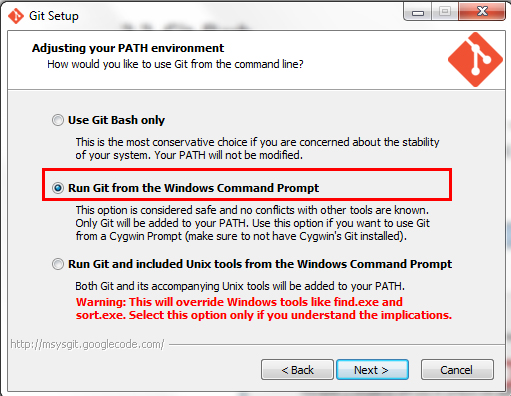
\includegraphics[width=6cm]{gitbash1.jpg}
	\caption{Command Context}
\end{figure}

\subsubsection{Line Endings}

The next screen lets one decide how file endings are pulled and committed. The iCampus Coding standards demand the Unix-style line endings. To this end only the second option is sufficient, because once style checking is enabled in your IDE the first and third options will, dependent on your system settings, report every single line of code as a breach of style, which removes any transparency whatsoever when searching for other errors.\\

\begin{figure}[h] 
	\centering
	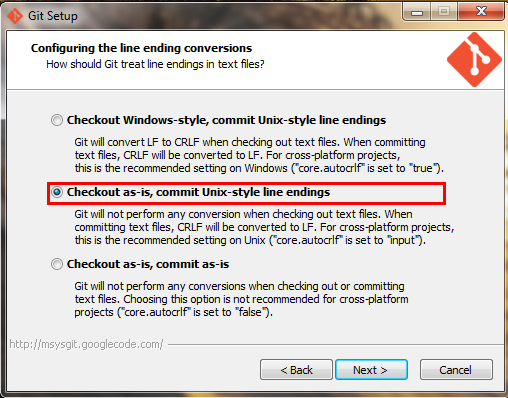
\includegraphics[width=6cm]{gitbash2.jpg}
	\caption{Line Endings}
\end{figure}

\subsection{User Configuration}

In order to take part in the development process you must take several steps to configure your user account.

\subsubsection{Global User Configuration}
In Git Bash the global user name and email must be set so that repository actions can be associated with a user.\\
\\
Start Git Bash and enter the following commands, replacing $<$First Name$>$, $<$Last Name$>$, and $<$Department$>$ with your first and last names and the abbreviation of the department in which you are matriculated.\\
\\
\begin{tabular}{l}
	\texttt{git config --global user.name "$<$First Name$>$ $<$Last Name$>$"}\\
	\texttt{git config --global user.email "$<$First Name$>$.$<$Last Name$>$@$<$Department$>$.thm.de"}\\
\end{tabular}\\
\\
You can confirm that the entries were saved correctly by entering the following command and comparing the associated values.\\
\\
\begin{tabular}{l}
	\texttt{git config -l}
\end{tabular}

\subsubsection{SSH-Key Creation}

After the user configuration is completed, an SSH-Key can be created using the following command in Git Bash.\\
\\ 
\texttt{ssh-keygen}\\
\\
The first question determines where the generated key will be saved and what its name will be. Per default this will be \textbf{\texttt{C:/Users/$<$Windows Account Name$>$/.ssh/id\_rsa}}. This directory is important for the next steps, as well as later when repositories are cloned. Press enter to confirm the default.
The next two questions will be to enter and confirm your password. You can also elect to have no password by pressing enter in answer to both questions.
\newpage
\section{PhpStorm}
\label{sec:PHP-Storm}

\subsection{Installation}
During the installation process you will be asked which file extensions should be associated with PhpStorm. As we use PhpStorm for the development with all given extensions, all can be selected. As of PhpStorm 8 this also allows for the editing of single files without the creation of a project.

\begin{figure}[h] 
	\centering
	\vspace{3pt}
	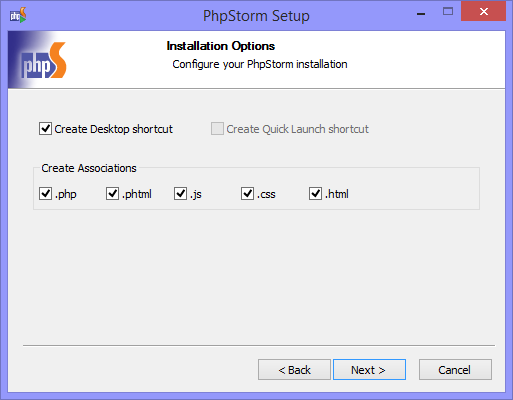
\includegraphics[width=5cm]{file-associations.png}
	\caption{File Associations}
\end{figure}

\noindent
For the most part the rest of the installation requires nothing special, however at the end you will be asked to chose between several themes and coloring/font style options. As this interface offers no preview it is best to go with the default settings. These selections can later be changed while running the PhpStorm which will actually show you what effects your selection has on its appearance.\\
\\
After the installation starting PhpStorm will request the lisence information. Please register at \url{https://www.jetbrains.com/shop/eform/students} as a student. After this procedure you can activate PhpStorm using your JetBrains account.

\begin{figure}[h]
	\centering
	\vspace{3pt}
	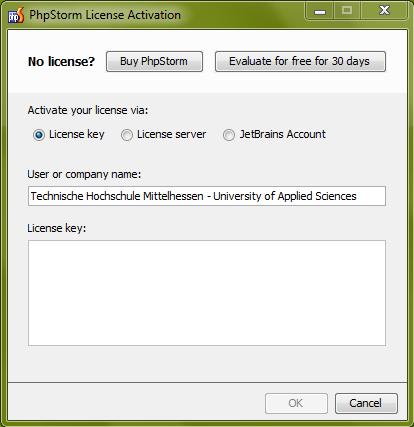
\includegraphics[width=4.5cm]{phpstorm-activation.png}
	\caption{PhpStorm License Activation}
\end{figure}

\newpage
\section{Code Sniffer and Mess Detector}
\label{sec:qatools}

PHP\_CodeSniffer is a PHP5 script that tokenises and ``sniffs" PHP, JavaScript and CSS files to detect violations of a defined coding standard. It is an essential development tool that ensures your code remains clean and consistent. It can also help prevent some common semantic errors made by developers.\footnote{\url{http://pear.php.net/manual/en/package.php.php-codesniffer.intro.php} Stand September 22, 2014}

\noindent
PHP Mess Detector on the other hand searches for problems more abstract and more serious such as\footnote{\url{http://phpmd.org/} Stand September 27, 2014}:

\begin{itemize}
	\item Possible bugs
	\item Suboptimal code
	\item Overcomplicated expressions
	\item Unused parameters, methods, properties
\end{itemize}

\subsection{Standards Directory Inclusion}
In order to use the Joomla standard you need to copy all data from \url{https://github.com/joomla/coding-standards} to the CodeSniffer standards folder: \newline
\texttt{C:\textbackslash xampp\textbackslash php\textbackslash pear\textbackslash PHP\textbackslash CodeSniffer\textbackslash Standards\textbackslash Joomla} (Windows)

\subsection{PhpStorm}

In order for Code Sniffer and Mess Detector to perform in PhpStorm they must first be integrated. This can be set as part of the default settings, meaning the settings will be applied to all projects, or in the project settings, where they would only valid for a specific project. The steps are exactly the same, but the entry point is slightly different. First access the settings using the menu item \texttt{File} and then selecting either \texttt{Default Settings...} or \texttt{Settings...} from the drop down menu.

\subsubsection{PhpStorm Inclusion}

To activate Code Sniffer click on \texttt{Languages \& Frameworks}, \texttt{PHP} and then \texttt{Code Sniffer} or \texttt{Mess Detector}. In the text field next to ``PHP Code Sniffer (phpcs) path" enter the path to phpcs.bat. In the standard installation this will be \texttt{C:\textbackslash xampp\textbackslash php\textbackslash phpcs.bat}. After you have input the path, click on \texttt{Validate}. If the file is valid, the you will be shown a short text containing the version of the installed Code Sniffer. Although not specifically stated the steps for Mess Detector inclusion are completely analogous.\\
\\
\begin{figure}[h] 
	\centering
	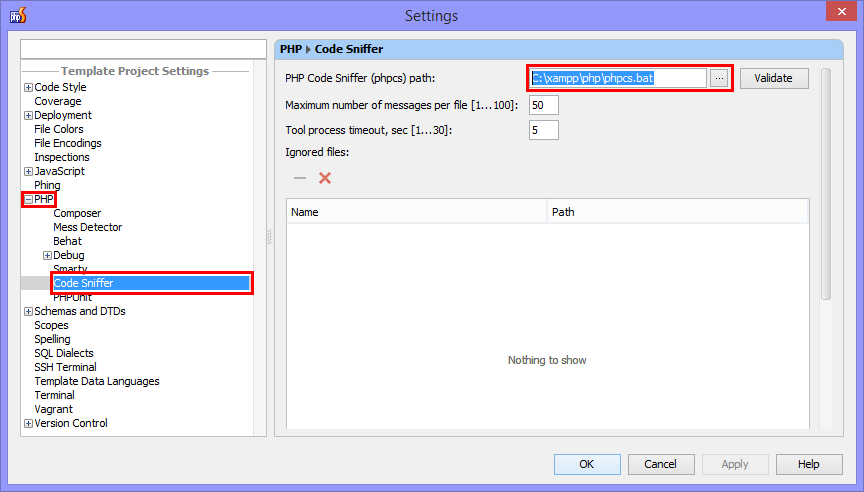
\includegraphics[width=14cm]{codesnifferinclusion.png}
	\caption{Code Sniffer - PhpStorm Inclusion}
\end{figure}

\subsubsection{PhpStorm Configuration}

Next we need to add PHP\_CodeSniffer to the inspections performed. With the settings still open, click on \texttt{Editor} then on \texttt{Inspections}, then in the list to the right \texttt{PHP}, and finally on \texttt{PHP Code Sniffer validation} to open the configuration settings for Code Sniffer.\\
\\
\begin{figure}[h] 
	\centering
	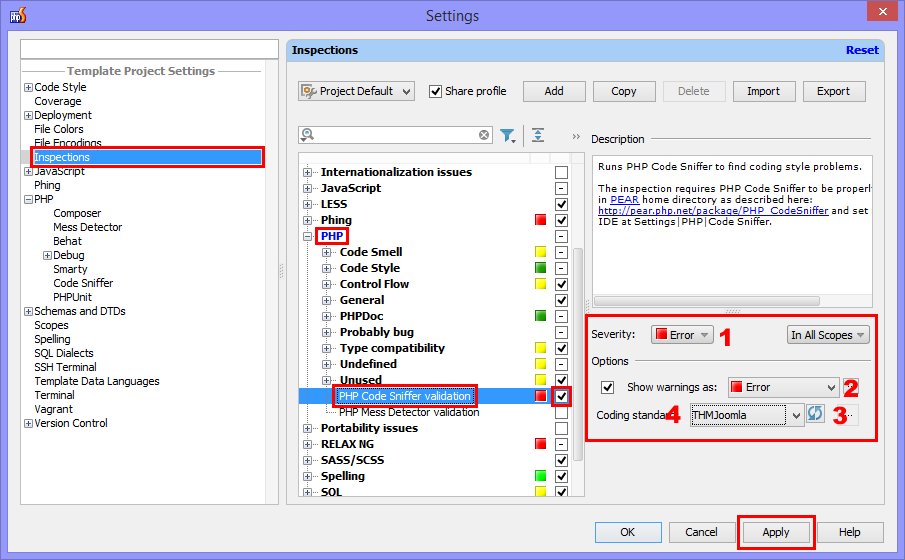
\includegraphics[width=14cm]{codesnifferconfiguration.png}
	\caption{Code Sniffer - PhpStorm Configuration}
	\label{fig:cspsc}
\end{figure}

\noindent
To activate the inspection we must first set the checkbox next to \texttt{PHP Code Sniffer validation}. This activation enables the further settings to the right which we see numbered with one through four in Figure \ref{fig:cspsc}.

\begin{enumerate}
	\item \texttt{Inspection severity}:``indicates how seriously the code issues detected by the inspection impact the project and determines how the detected issues should be highlighted in the editor."\footnote{http://www.jetbrains.com/phpstorm/webhelp/configuring-inspection-severities.html Stand September 22, 2014}
	\item \texttt{Display severity}: defines how the infractions found are marked.
	\item \texttt{Refresh}: updates the list of available coding standards. Should the desired standard not be found in the folder defined in the section on symbolic links, you can also manually search for the standard on your file system.
	\item \texttt{Available standards}: a list of standards found. In iCampus we use the THM Joomla Standard which inherits or extends many of the definitions in the Joomla standard.
\end{enumerate}

\noindent
It is recommended that both inspection and display severity be set to errors to make the standard infractions more noticable. Settings take effect when the \texttt{Apply} button has been pressed.\\
\\
Inspection settings for Mess Detector are also analogous here, with the distinction that one need not select a standard, instead selecting which rule sets should be applied.
\newpage

\section{Joomla!}
\begin{quote}
	Joomla is an award-winning content management system (CMS), which enables you to build Web sites and powerful online applications. Many aspects, including its ease-of-use and extensibility, have made Joomla the most popular Web site software available. Best of all, Joomla is an open source solution that is freely available to everyone.\footnote{\url{http://www.joomla.org/about-joomla.html} Stand 27 September, 2014}
\end{quote}

\subsection{Joomla! 3.x Development}
First extract the archive file downloaded from \href{http://www.joomla.org/download.html}{the Joomla! website} and give it a URL friendly name such as ``j3". Next place this folder in your web directory. If you followed the default installation steps this should be located at \texttt{C:\textbackslash xampp\textbackslash htdocs}.\\
\\
Open a browser of your choosing and enter \texttt{localhost/$<$Your Joomla 3.x Folder$>$} in the address bar. If you renamed the backup ``j3" this would then be \url{localhost/j3}. This will open the main configuration page as seen in Figure \ref{fig:j3mainconfiguration}.

\newpage

\begin{figure}[h] 
	\centering
	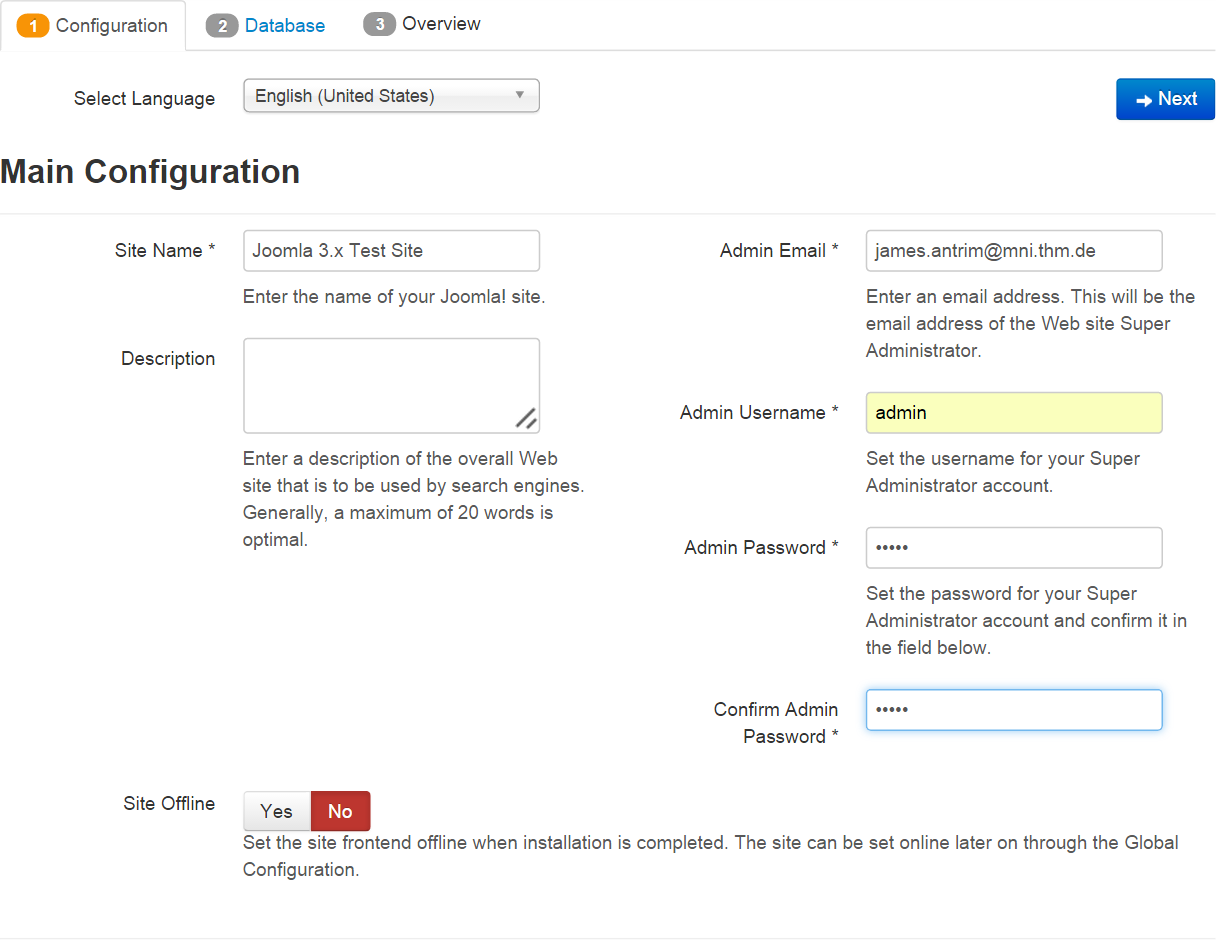
\includegraphics[width=8cm]{j3mainconfiguration.png}
	\caption{Joomla Main Configuration}
	\label{fig:j3mainconfiguration}
\end{figure}

\noindent
Here you will need to enter the \texttt{Site Name}, \texttt{Admin Email}, \texttt{Admin Username}, \texttt{Admin Password}, and \texttt{Confirm Admin Password}. Click ``$\Rightarrow$ Next" to move on to the database configuration.\\

\begin{figure}[h] 
	\centering
	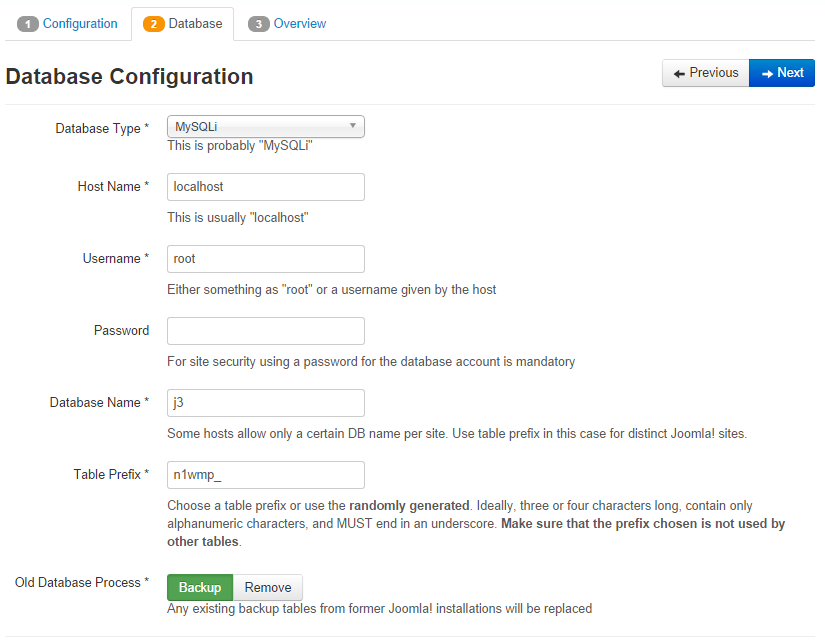
\includegraphics[width=8cm]{j3databaseconfiguration.png}
	\caption{Joomla Database Configuration}
	\label{fig:j3databaseconfiguration}
\end{figure}

\noindent
Use the following values to complete the form, then click ``$\Rightarrow$ Next" to continue on to the finalization.\\
\\
\begin{tabular}{l l}
	\texttt{Database type} & MySQLi\\
	\texttt{Host Name} & localhost\\
	\texttt{Username} & root\\
	\texttt{Password} & (empty, unless set)\\
	\texttt{Database name} & j3 (unless named otherwise)\\
\end{tabular}

\newpage

\begin{figure}[h]
	\centering
	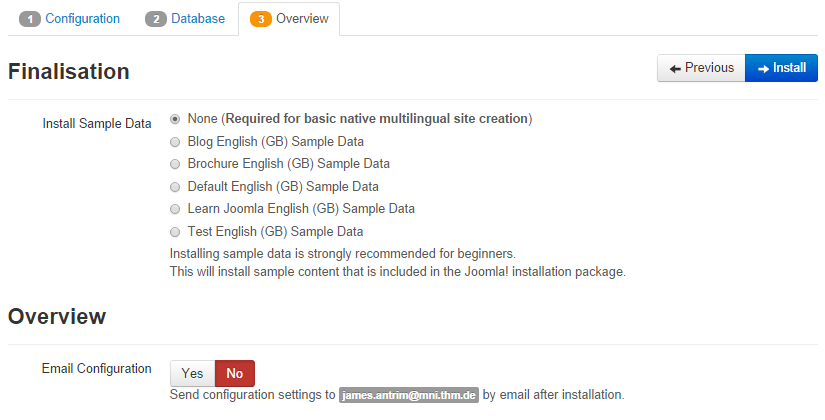
\includegraphics[width=10cm]{j3finalization.png}
	\caption{Joomla Finalization}
	\label{fig:j3finalization}
\end{figure}

\noindent
Here you can choose whether or not you wish to install sample data. Leave ``None" selected and click ``$\Rightarrow$ Install" to complete the installation. The installation will then show the progress of the database construction. When this is finished you will be told that Joomla! is installed. You should now press the orange button ``Remove installation folder" to complete the installation. You can choose to visit the frontend or backend of the site by clicking the appropriate button.
